% PROGETTO BASI DI DATI 2015 , MERLINO GIUSEPPE is CEO and VIOLETTO MIKI is SGUATTERO
%
% stato della relazione :
%
% abstract da rileggere e forse modificare
% analisi dei requisiti da cambiare un bel pò, aspetterei di farlo dopo aver fatto la progettazione concettuale, almeno l'inizio
% progettazione concettuale rimodellata, da rileggiere da capo, molte frasi da migliorare che sicuramente ho scritto cazzate
% immagini cominciate a fare
%
\documentclass[a4paper,twoside]{article}

\usepackage[margin=3cm]{geometry}
\usepackage[utf8]{inputenc}
\usepackage[main=italian, english]{babel}
\usepackage{graphicx}
\usepackage{rotating}
\usepackage{verbatim}
\usepackage{listings}
\usepackage[colorlinks=true,linkcolor=black,urlcolor=blue]{hyperref} % ancore delle varie sezioni sul menu

%\graphicspath{Immagini/} %non va ... bho

\author{Giuseppe Merlino,Miki Violetto}
\title{Relazione progetto BiciRent}
\date{\today}

\begin{document}
\maketitle

\newpage
\tableofcontents
\newpage
\listoffigures
\newpage

%  link utili
%  http://www.goodbikepadova.it/Default.aspx : GoodBike, dove prendiamo spunto per il progetto
%  www.lucidchart.com : programma per fare i grafici dei schemi concettuale e logico

\section{Abstract}
BiciRent è un servizio di bike sharing ispirato a Goodbike presente qui a Padova.\newline
Permette grazie ad una tessera personale di noleggiare in qualsiasi momento una delle bici presenti in apposite stazioni collocate in diverse aree della città ed utilizzarla per muoversi, lasciandola poi in un'altra stazione dove sia presente un posto libero.\newline
La tessera ha validità specifica a seconda del piano che si sottoscrive, e sono previsti sconti per studenti e turisti.\newline
Le biciclette noleggiabili sono di due tipi, quella classica munita di un passeggino oppure quella a pedalata assistita.\newline
Le stazioni sono presenti in molti aree della città e sono munite di sicure automatiche antifurto. Saranno sempre presenti biciclette da noleggiare e posti per lasciare la bici noleggiata grazie ad un servizio di trasporto e le biciclette rotte verranno sostituite da nuove.\newline
Il servizio tende ad essere automatizzato e permette all'abbonato di controllare facilmente se in una data stazione siano presenti biciclette o ci siano posti vuoti per depositare la bici noleggiata. Può segnalare la presenza di guasti delle biciclette.\newline
Si prospettano circa 1700 noleggi giornalieri e una media di 200 richieste d'intervento al giorno (mancanza di bici e rotture); inoltre viene richiesta la composizione dei posti di ogni singola stazione (presenza biciclette, tipi disponibili e posti liberi) almeno 3000 volte ogni giorno, ma con punte di quasi 900 richieste in una singola mezz'ora (ad esempio nelle ore di punta).

\section{Descrizione testuale dei requisiti e operazioni tipiche}
%Alias analisi dei requisiti XD
Si vuole realizzare una base di dati e una semplice applicazione web che contenga e gestisca le informazioni relative al bike sharing, simulando inoltre le operazioni che è possibile eseguire tramite la colonnina.

\subsection{Descrizione testuale}
Sono necessarie le informazioni personali degli utenti per permettergli di registrarsi e comprare una tessera; saranno quindi obbligatori nome e cognome, la data e il luogo di nascita, le informazioni sulla residenza (via, numero civico, città, C.A.P.) e un indirizzo email, l'utente può inserire il suo numero telefonico (campo facoltativo) per ricevere ulteriori informazioni.\newline
Per poter poi usufruire di convenzioni rilasciate solo a studenti, sarà necessario il codice di matricola in caso di universitari o l'id della carta Io Studio, e le agevolazioni verranno fornite solo per abbonamenti da mensili in su.\newline
Nel caso di turisti non è necessaria nessuna informazione aggiuntiva, ma l'agevolazione verrà fornita solo ai piani giornalieri, weekend o settimanali.\newline
La tessera personale, che verrà utilizzata per identificare l'utente in tutte le operazioni che effettuerà, avrà una validità data dal piano presente (giornaliera, per un singolo fine settimana (sabato e domenica), oppure essere collegata ad un abbonamento di varie taglie: settimanale, mensile, trimestrale, semestrale o annuale) e non potrà mai rimanere senza piano. Un utente con piano ancora valido (attivo) potrà usufruire di tutti i servizi, mentre un utente con una tessera non più valida (piano scaduto) potrà solo comprare un nuovo piano ad un prezzo prefissato, da cui verrà tolto il 15\% per i turisti che usufruiscono dell'agevolazione e del 10\% per gli studenti.\newline
Le biciclette, identificate da un id univoco, possono essere a pedalata assistita (elettriche) oppure con un seggiolino (la maggior parte), mentre in base al loro stato possono essere suddivise tra biciclette in uso, cioè che possono essere noleggiate o che stanno venendo noleggiate, biciclette in deposito o biciclette danneggiate; lo stato di una bicicletta non sempre corrisponde alla propria posizione, infatti una bici danneggiata può sia essere presente in magazzino che presso una colonnina.\newline
La  colonnina, identificata da un codice numerico e dalla stazione di cui fa parte, presenta uno stato,  libera o occupata a seconda della presenza o meno di una bicicletta, oppure danneggiata se la colonnina o la bici presente sono danneggiate.\newline
Una stazione é formata da più colonnine e si utilizza anche in questo caso un id per l'identificazione; avrà un attributo contenente l'indirizzo di ubicazione, per facilitare la ricerca nelle mappe. L'utente interagirà con la stazione per conoscere gli stati delle varie colonnine (ma non si interesserà del singolo stato di ogni colonnina).

\subsection{Operazioni tipiche}
Operazioni tipiche eseguite dall'utente :
\paragraph{Noleggio di una bicicletta} Il noleggio interessa una bici con stato "in uso" che sta attualmente occupando una colonnina perché non è già in noleggio, e lascia la colonnina nello stato di libera. Questo genera un noleggio di tipo in corso, dove viene salvata la bicicletta, la colonnina di prelievo e l'orario di prelievo. Un utente può avere un singolo noleggio attivo alla volta.
\paragraph{Deposito di una bicicletta} Il deposito di una bicicletta interessa sempre una bicicletta con lo stato in uso, e modifica un noleggio di tipo in uso in uno di tipo terminato, salvando quindi la colonnina in cui viene depositata la bicicletta e l'orario di deposito; questo porta la colonnina, che prima era nello stato libera, nello stato occupata.
\paragraph{Controllo dello stato di una stazione o area} Il controllo dello stato implica un controllo di ogni singola colollonina, e ritorna quanti spazi, liberi e quante biciclette e di quale tipo sono presenti sulla data stazione , per l'area si cerca in tutte le stazioni di quell'area.
\paragraph{Segnalazione di mancanza di biciclette o spazi vuoti} Una segnalazione di tipo mancanza viene chiamata dall'utente tramite il sito oppure il numero telefonico su una data stazione e comporterà uno o più trasporti per assolvere la segnalazione.
\paragraph{Segnalazione di rottura} Una segnalazione di rottura viene chiamata dall'utente da una singola colonnina o dal sito e comporterà un ordine di manutenzione che potrà interessare la colonnina o la bicicletta.
\par Operazioni tipiche non effettuate dall'utente :
\paragraph{Trasporto di una bicicletta} Il trasporto può avvenire perché segnalato da un utente oppure per esigenze interne, e comporta il movimento di una bicicletta in tre modi diversi: tra due colonnine di diverse stazioni, dal magazzino ad una colonnina oppure da una colonnina al magazzino. Il trasporto di una bicicletta cambia sicuramente lo stato della colonnina interessata, e forse cambia anche lo stato della bicicletta.
\paragraph{Manutenzione di una colonnina o di una bicicletta} La manutenzione può avviene a seguito di una segnalazione oppure può essere richiesta dall'azienda e prevede un controllo della bicicletta o della colonnina, che verrà riassunto in una descrizione dei danni presenti che sono stati riparati, e dall'orario di fine manutenzione. Si nota che la manutenzione di una bicicletta interessa la colonninna su cui è stata presente, e che per semplicità ed efficienza viene sempre controllata sia la colonnina che la bicicletta se presente.Un'operazione di matunenzione comporterà per la colonnina e la bicicletta un cambio di stato (erano daneggiate, ora non lo sono più).
\par Operazioni dell'area amministrativa :
\paragraph{resoconto dei lavori di manutenzione} E' visibile dall'area amministrativa un resoconto dei lavori di manutenzione alle biciclette e alle colonnine dello scorso mese. Con riportati le date e gli orari.
\paragraph{storico di una bicicletta} Può venire richiesto dall'area amministrativa le manutenzioni di una bicicletta, come gli utenti che l'hanno noleggiata e il tempo in cui è stata noleggiata.
\paragraph{lista dei mezzi danneggiati} Può venire richiesta una lista delle biciclette danneggiate, con la stazione e l'area in cui sono presenti.

\subsection{Nuovi requisiti}
Dopo un'esposizione e un ragionamento sulle operazioni da eseguire, si possono delineare delle prime modifiche da effettuare alla descrizione testuale :
\paragraph{Operazioni di diverso spessore} Si nota che operazioni quali noleggio-deposito, segnalazione, trasporto e manutentione non sono semplici operazioni unitarie, ma coinvolgono molteplici operazioni.
\paragraph{modifica dello stato della bicicletta} Lo stato di una bicicletta non può venire rappresentato solo con in uso, in magazzino o danneggiata; Si decide di utilizzare 2 caratteristiche : lo stato della bicicletta (operativa o danneggiata) e la sua posizione (magazzino o in uso); Questo comporta un miglior rappresentazione dello stato della bicicletta.
\paragraph{Realtà su due livelli} Si nota che si potrebbe dividere la realtà d rappresentare in due parti: una parte si occupa dello stato attuale del sistema, quindi di dove attualmente sono le bici, della presenza di collonnine vuote o piene, etc mentre un'altra si occupa dello storico di queste informazioni, quindi dei noleggi terminati, dei trasorti effettuati, delle manutenzioni, etc.

\section{Progettazione concettuale}
%top-down , bottom-up, inside-out , misto
Per la modellazione concettuale decido di partire dall'operazione principale del sistema che stiamo modellando, il noleggio.
Il noleggio, visto come l'azione che va da quando si preleva una bicicletta da una colonnina a quando la si deposita, è uno stato presente del sistema; ma possiamo assocciare a noleggio una caratteristica di storico dei noleggi, che corrispondo ai tutti i noleggi che sono stati effettuati, non solo quelli in corso.

\subsection{Entità Noleggio}
L'entità \textbf{Noleggio} rappresenta il singolo noleggio effettuabile dall'utente.\newline
Attributi di Noleggio :
\begin{itemize}
 \item utente
 \item bicicletta
 \item colonnina prelievo
 \item orario prelievo
 \item data prelievo
 \item colonnina deposito
 \item orario deposito
 \item data deposito
\end{itemize}
%immagine ConNoleggio01
Osservando gli attributi si può trovare una suddivisione dell'entità Noleggio, tra noleggi in corso e terminati.\newline
L'entità \textbf{Noleggio in corso} è un sottoinsieme di Noleggio.\newline
Attributi di Noleggio in corso :
\begin{itemize}
 \item orario prelievo
 \item data prelievo
 \item colonnina prelievo
\end{itemize}
L'entità \textbf{Noleggio terminato} è un sottoinsieme di Noleggio.\newline
Attributi di Noleggio terminato :
\begin{itemize}
 \item orario deposito
 \item data deposito
 \item colonnina deposito
\end{itemize}
Noleggio è quindi una generalizzazione completa ed esclusiva dei sottoinsiemi Noleggio in corso e Noleggio terminato.\newline
L'entità \textbf{Noleggio} risultante ha quindi come attributi :
\begin{itemize}
 \item utente
 \item bicicletta
\end{itemize}
%immagine ConNoleggio02

\subsection{Entità Utente}
L'entità \textbf{Utente} rappresenta la persona che effettua i noleggio, e più avanti anche altre cose (segnalazioni per esempio).\newline
Attributi di Utente :
\begin{itemize}
 \item nome
 \item cognome
 \item data di nascita
 \item luogo di nascita
 \item indirizzo di residenza(via e numero)
 \item città di residenza
 \item cap
 \item email (può essere nullo)
 \item numero telefonico (può essere nullo)
 \item tessera
\end{itemize}
L'entità \textbf{Studente} è un sottoinsieme di Utente.\newline
Attributi di Studente :
\begin{itemize}
 \item matricola
\end{itemize}
L'entità \textbf{Turista} è un sottoinsieme di Utente.\newline
Utente è quindi una generalizzazione parziale esclusiva delle specializzazioni Studente e Turista.
%immagine ConUtente01

\subsection{Relazione NomeRelazioneboo}
Relazione tra Utente e Noleggio : \textbf{NomeRelazioneboo}.\newline
Un Utente può effettuare da 0 a N noleggi, mentre ogni Noleggio viene effettuato da 1 e solo 1 Utente.
%immagine ConNomeRelazioneboo01

\subsection{Entità Tessera}
l'Entità : \textbf{Tessera} rappresenta la tessera personale in possesso di ogni singolo utente.\newline
Attributi di Tessera :
\begin{itemize}
 \item codice tessera (chiave)
 \item data sottoscrizione abbonamento
 \item abbonamento
\end{itemize}
%immagine ConTessera01

\subsection{Relazione Tesseramento}
Relazione tra Utente e Tessera : \textbf{Tesseramento}.\newline
Un Utente può avere una sola Tessera, e la Tessera avrà come proprietario quell'unico Utente.\newline
Mi accorgo che quando ci si riferisce ad Utente, la maggior parte delle volte ci si riferisce alla sua tessera, questo è possibile in quanto Tesseramento ha una cardinalità 1:1 : queste volte verrà usata tessera per esempio con NomeRelazioneboo.
%immagine ConTesseramento01

\subsection{Relazione NomeRelazioneboo modificata}
Relazione non più tra Utente e Noleggio ma tra Tessera e Nolaggio: \textbf{NomeRelazioneboo}.\newline
Una Tessera può effettuare da 0 a N noleggi, mentre ogni Noleggio viene effettuato da 1 e solo 1 Tessera.
%immagine ConNomeRelazioneboo02

\subsection{Entità Piano}
Entità : \textbf{Piano} rappresenta la validità con cui la tessera è valida.\newline
Attributi di Piano :
\begin{itemize}
 \item tipologia : giornaliero, weekend, settimanale, mensile, trimestrale, semestrale o annuale
 \item costo
\end{itemize}
%immagine ConPiano01

\subsection{Relazione Abbonamento}
Relazione tra Tessera e Piano : \textbf{Abbonamento}.\newline
Una Tessera ha 1 e 1 solo piano, mentre un Piano può essere sottoscritto da 0 a N tessere.
%immagine ConAbbonamento01

\begin{figure}[h]
 \centering
  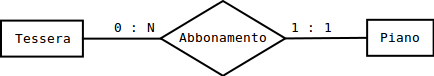
\includegraphics[width=0.5\textwidth]{Immagini/ConAbbonamento01}
\caption{}
\end{figure} 




\subsection{Entità Bicicletta}
Entità : \textbf{Bicicletta} rappresenta la bicicletta noleggiabile dall'utente.\newline
Attributi di Bicicletta :
\begin{itemize}
 \item codice identificativo (chiave)
 \item tipo : normali o pedalata assistita
 \item stato attuale (
\end{itemize}
%immagine ConBicicletta01
Lo stato attuale della bicicletta potrebbe restare espesso come un attributo, ma per rappresentare meglio le relazioni che interessano non solo Bicicletta e Noleggio, ma anche il concetto di Segnalazione espresso più avanti, si procede con una serie di sottoinsiemi.\newline
Entità \textbf{Bicicletta attiva} è un sottoinsieme di Biciclette che rappresenta le biciclette in stato attivo, cioè noleggiate o noleggiabili.\newline
Entità \textbf{Bicicletta danneggiata} è un sottoinsieme di Biciclette che rappresenta le biciclette danneggiate, cioè che non possono venire noleggiate e necessitano di una manutentione.\newline
Entità \textbf{Bicicletta ferma} è un sottoinsieme di Biciclette che rappresenta le biciclette in magazzino, cioè biciclette che non sono in servizio al momento.\newline
Bicicletta attiva, Bicicletta danneggiata e Bicicletta ferma sono sottoinsiemi globali esclusivi di Bicicletta.\newline
%immagine ConBicicletta02
NB :\newline
Si può notare ora che si sono aggiunti dei sottoinsiemi di Bicicletta come l'attributo bicicletta di Noleggio debba essere cambiato : infatti un Noleggio in corso sarà effettuato su una Bicicletta attiva, mentre un Noleggio terminato può interessare una Bicicletta in qualsiasi stato attuale, essendo stato terminato nel passato.

\subsection{Relazione Prelievo}
Relazione tra Bicicletta attiva e Noleggio in corso : \textbf{Prelievo}.\newline
Possiamo togliere da noleggio degli attributi propri di Prelievo :
\begin{itemize}
 \item orario prelievo
 \item data prelievo
 \item colonnina prelievo
\end{itemize}
Una Bicicletta attiva può avere 1 solo Noleggio al massimo, e un Noleggio in corso interessa 1 e 1 soltato Bicicletta Attva.
%immagine ConPrelievo01

\subsection{Relazione Deposito}
Relazione tra Bicicletta e Noleggio terminato : \textbf{Deposito}.\newline
Possiamo togliere da noleggio degli attributi propri di Deposito :
\begin{itemize}
 \item orario deposito
 \item data deposito
 \item colonnina deposito
\end{itemize}
Una Bicicletta può avere da 0 a N Noleggi terminati, ma un Noleggio terminato interesse sempre e solo 1 Bicicletta.7
%immagine ConDeposito01

\subsection{Entità Noleggio modificata}  %porta allo 'schema ragionamento 2'
Tutte queste modifiche portano ad una modifica sostanziale dell'entità Noleggio.\newline
Ci si occorge che quello che chiamiamo Noleggio altro non è che un Noleggio in corso, e che un Noleggio terminato è un sottoinsieme di un Noleggio in corso, con l'aggiunta delle informazioni del deposito.
Quindi la nuova entità \textbf{Noleggio} ha come relazioni :
\begin{itemize}
 \item con tessera ha NomeRelazioneboo
 \item con bicicletta dovrei avere Prelievo, che però deve essere modificata
\end{itemize}
Come sottoinsieme di Noleggio ho \textbf{Noleggio terminato}, che presenta la relazione deposito.\newline
Dopo questa modifica bisogna riflettere sulle relazioni Prelievo e Deposito : in ogni singola ennupla la Bicicletta coinvolta in entrambe le relazioni è la stessa, le cose che differiscoso sono alcuni attributi (orario, data e colonnina interessati) e che Prelievo relaziona con il sottoinsieme Bicicletta attiva, e non la generalizzazione Bicicletta.\newline
Da questo punto di vista la  modifica che si andrebbe necessariamente a fare renderebbe il modello più debole, in quanto si andrebbe a togliere il vincolo che lega un Noleggio in corso con una Bicicletta attiva, portandolo su Bicicletta.\newline
Un'altro aspetto da discutere è dove inserire gli attrubiti data, ora e colonnina : se si unissero le relazioni si potrebbe scegliere di metterli come attributi sulle entità Noleggio e Noleggio terminato, in quanto le relazioni hanno cardinalita 1 : 1 con Bicicletta e Bicicletta attiva.\newline
Altro punto favorevole all'unione delle due relazioni è l'analisi dell'attributo colonnina, che si può intuire verrà espresso in una relazione con un'entità colonnina ancora da modellare (in quanto colonnina presenta altre informazioni da modellare), quindi Prelievo e Deposito diventerrano relazioni tra Noleggio e colonnina.\newline
Quindi Noleggio avrà come relazioni :
\begin{itemize}
 \item con Tessera rimane NomeRelazioneboo
 \item con Bicicletta avrà una relazione
 \item con Colonnina avro una relazione Prelievo, ancora da modellare
\end{itemize}
Il sottoinsieme di Noleggio sarà l'entità \textbf{Noleggio terminato} che avrà :
\begin{itemize}
 \item una relazione con Colonnina chiamata Deposito
\end{itemize}
Si può vedere questa modifica come una semplificazione delle due relazioni ternarie che sarebbero risultate tra Noleggio, Bicicletta e Colonnina.
%immagine ConNoleggio03

\subsection{Relazione Noleggio-Bicicletta}
La relazione \textbf{Noleggio-Bicicletta} interessera La Bicicletta e il Noleggio in cui viene noleggiata.\newline
Una Bicicletta può essere noleggiata da 0 a N volte, mal un noleggio interessa sempre e solo 1 bicicletta.
%immagine ConNoleggio-Bicicletta01

\subsection{Entità Colonnina}
L'entità \textbf{Colonnina} rappresenta il luogo dove la bicicletta viene prelevata e successivamente depositata.\newline
Attributi di Colonnina :
\begin{itemize}
 \item codice numerico
 \item stazione (che rappresenta il dove)
 \item stato (danneggiata oppure sana)
\end{itemize}
Una caratteristica della colonnina é la possibilità di essere considerata libera oppure occupata : una colonnina occupata differisce da una colonnina libera in quanto occupata da una bicicletta, quindi in relazione con l'Entità Bicicletta.
Le colonnine occupate fanno parte del sottoinsieme \textbf{Colonnina occupata} che non presenta nessun attributo ma solo una relazione con la bicicletta che al momento è presente.
%immagine ConColonnina01

\subsection{Relazione Posizione}
La relazione \textbf{Posizione} collega la Bicicletta attiva con la Colonnina occupata su cui è possibile trovarla.\newline
Una Bicicletta attiva può essere presente al massimo su una Colonnina occupata (0 : 1) mentre una Colonnina occupata ha presente una Bicicletta attiva (0 : 1).
%immagine ConPosizione01

\subsection{Relazione Prelievo modificata}
La relazione \textbf{Prelievo} collega il Noleggio con la Colonnina in cui è stata prelevata la Bicicletta.\newline
Attributi di Prelievo :
\begin{itemize}
 \item orario prelievo
 \item data prelievo
\end{itemize}
Una Colonnina può avere da 0 a N prelievi, mentre un Noleggio ha sempre e solo 1 prelievo.\newline
Si nota come Prelievo influisce sulla Colonnina : un'istanza della relazione Prelievo può venire invocata solo su una Colonnina considerata occupata, facendola diventare libera, cioè rimuovendo in quella specifica ennupla di colonnina la relazione Posizione al momento della creazione della relazione Prelievo.
%immagine ConPrelievo02

\subsection{Relazione Deposito modificata}
La relazione \textbf{Deposito} è simile alla relazione prelievo e collega la Colonnina con il Noleggio terminato che ha depositato lì la Bicicletta.\newline
Attributi di Deposito :
\begin{itemize}
 \item orario deposito
 \item data deposito
\end{itemize}
Una Colonnina può avere da 0 a N depositi, ma un Noleggio terminato ha sempre e solo 1 deposito.\newline
Come per prelievo si nota che un deposito può avvenire solo su una Colonnina considerata libera, e conseguentemente provoca la creazione di una relazione Posizione nella ennupla interessata.
%immagine ConDeposito02

\subsection{Entità Stazione}
L'entità \textbf{Stazione} rappresenta un gruppo di più colonnine fisicamente nella stessa zona.\newline
Attributi di \textbf{Stazione} :
\begin{itemize}
 \item codice identificativo (chiave)
 \item indirizzo (via e numero)
 \item postazioni presenti (numero di colonnine)
 \end{itemize}
%immagine ConStazione01

\subsection{Relazione Appartenenza}
La relazione \textbf{Appartenenza} associa le colonnine con la propria stazione a cui appartengono.\newline
Una colonnina appartiene necessariamente a soltanto 1 stazione, mentre la stazione ha più colonnine (1 : N).
%immagine ConAppartenenza01

\subsection{Relazione Segnalazione di rottura}
La relazione \textbf{Segnalazione di rottura} associa l'utente che la effettua con la colonnina segnalata e in alcuni casi la Bicicletta presente.\newline
Una tessera può compiere da 0 a N segnalazioni di rottura, mentre una Segnalazione di rottura viene eseguita da 1 tessera al massimo.\newline
Si nota come una volta inserita la segnalazione lo stato della Colonnina e della Bicicletta che la occupa (se presente) cambi e diventi danneggiata.
%immagine ConSegnalazione di rottura01

\subsection{Relazione Segnalazione di mancanza}
La relazione \textbf{Segnalazione di mancanza} associa l'utente che la effettua con la Stazione che segnala, manifestando la necessità di un trasporto (sia per mancanza di colonnine libere, che per mancanza di biciclette d noleggiare (colonnine occupate).\newline
Una tessera può effettuare da 0 a N segnalazioni di mancanza, ma una stazione può avere al più 1 segnalazione.
%immagine ConSegnalazione di mancanza01

\subsection{Entità Manutenzione}
L'entità \textbf{manutentione} rappresenta lo storico delle manutenzioni sulle colonnine o biciclette e ha come attributi :
\begin{itemize}
 \item data del completamento
 \item descrizione del danno riparato
\end{itemize}
A seconda di cosa ha subito la manutenzione si avranno due sottoinsiemi \textbf{bicicletta} e \textbf{colonnina}, quindi Manutenzione sarà una generalizzazione globale esclusiva.
%immagine ConManutenzione01

\subsection{Relazione Manutenzione bicicletta-Bicicletta}
La relazione \textbf{Manutenzione bicicletta-Bicicletta} associa ogni singolo lavoro di manutentione alla bicicletta che l'ha subito.\newline
Ogni Bicicletta può subire da 0 a N lavori di manutentione mentre ogni lavoro di manutenzione bicicletta è stato fatto su una singola bicicletta.
%immagine ConManutenzione bicicletta-Bicicletta01

\subsection{Relazione Manutenzione colonnina-Colonnina}
La relazione \textbf{Manutenzione colonnina-Colonnina} associa ogni singolo lavoro di manutentione alla colonnina che l'ha subito.\newline
Ogni Colonnina può subire da 0 a N lavori di manutentione mentre ogni lavoro di manutenzione colonnina è stato fatto su una singola colonnina.
%immagine ConManutenzione colonnina-Colonnina01

\subsection{Entità Trasporto}
L'entità \textbf{Trasporto} rappresenta lo storico dei trasporti effettuati per muovere una singola Bicicletta con attributi :
\begin{itemize}
 \item data
 \item numero viaggio
\end{itemize}
In realtà esistono tre tipi di trasporto in base a dove si preleva la bicicletta e dove la si deposita (da non confondere con l'azione dell'utente, questi sono trasporti interni).\newline
Un sottoinsieme \textbf{movimento} è un trasporto che interessa 2 colonnine : si preleva da una e la si deposita nell'altra.\newline
Un sottoinsieme \textbf{aggiunta} è un trasporto che interessa una sola colonnina : si prende la Bicicletta dal magazzino e la si deposita in una Colonnina.\newline
Un altro sottoinsieme \textbf{rimozione} è un trasporto che interessa anch'esso solo una colonnina : si preleva la Bicicletta dalla Colonnina e la si deposita dal magazzino.\newline
Si nota come tutti questi trasporti provochino un cambio di stato della Colonnina; inoltre rimozione e aggiunta modificano anche lo stato della Bicicletta.
%immagine ConTrasporto01

\subsection{Relazione Trasporto-Bicicletta}
La relazione \textbf{Trasporto-Bicicletta} assoccia ad ogni singolo Trasporto la Bicicletta trasportata.\newline
Una Bicicletta piò subire da 1 a N trasporti (inizialmente la si estrae dal magazzino, quindi la si aggiunge), mentre un Trasporto trasporta 1 e una soltanto Bicicletta.
%immagine Con Trasporto-Bicicletta

\subsection{4 Relazioni Trasporto-Colonnina}
Da finire

\section{Progettazione logica}

\section{Implementazione dello schema logico}

\section{Query, procedure, trigger e funzioni}

\section{Interfaccia web}

\end{document}